%\emph{
%Author(s):   S. Aoudia, L. Bosi, L. Storchi,  \\
%}
\dots

\FloatBarrier
\subsection{Computing Challenges}

In this section we try to use our trend analysis and our simulations in order to foresee for the next 12-14 years the computing solutions and power gain.  
%\FloatBarrier
%\subsubsection{Moore's law}

%''Moore's Law is a violation of Murphy's Law. Everything gets better and better'' ~\cite{MooreFrase2} 
%("Moore's Law at 40 . Happy birthday". The Economist. 2005-03-23. http://economist.com/displaystory.cfm?storyi\_id=3798505. Retrieved 2006-06-24)
% this is how Gordon Moore 
%commented the law, that bears his name, in 2005. Moore's law describes trend in the history of computing 
%hardware. The law has been originally thought to describes the number of transistors that can be placed 
%inexpensively on an integrated circuit. But now we see this law can be applied also to the capabilities 
%of many digital electronic devices, such as memory capacity, sensors and even even the number and size 
%of pixels in digital cameras. There are in fact many other laws related to the Moore's one. Other laws 
%prediction for example hard disk storage cost per unit of information, or network capacity, or pixels 
%per dollar, and more.
%
%Gordon E. Moore formulated the law by a simple observation. In 1965 he noted that number of components 
%in integrated circuits had doubled every two years from the invention of the integrated circuit in 1958. Thus, he predicted that the trend would continue  ''for at least ten years''. Years after the law has been 
%reformulated to take into account an higher growth, and the final formulation state that integrated circuits 
%would double in performance every 18 months. Thus ''Moore's first law predict'' an exponential rates for the transistor counts in a microprocessor: $P_n = P_0 \cdot 2^n$, where $P_n$ is the predicted computer processing power in 
%future years, $P_0$ is the actual computer processing power, and $n$ the number of years divided by the doubling period, expressed in years. i.e.\ if we consider the transistor count the doubling factor is 2 (every 2 years), while if we consider the processors speed the doubling factor is 1.5 (every 18 months).
%
%Moore's first law can be viewed just as an observation, but maybe there is even more. Maybe behind 

%it there is a more deeper law, a law driving evolution of information and technology, of which the 
%Moore's law is just a consequence. But up to now what it is clear is that this law has been 
%widely accepted, and is used as a goal for both marketing and engineering departments of semiconductor 
%manufacturers. We recall what has been reported in the previous section about top500 trend, that confirms the Moore's law. 

What about future trends? As we are writing, also within computer 
industry technology's road map ``believes Moore's Law will continue to hold good through 2029'',  citing Pat Gelsinger, SVP and co-GM of Intel's Digital Enterprise Group (DEG)~\cite{IntelCite}.

%Although specialists agree that by 2019 the current strategy of ever-finer photolithography will 
%have run its course, it is likely that some new type of technology will replace current
%integrated-circuit technology, and that Moore's Law will hold true long after 2020. 
%New type of technology like optical or quantum computers, 
Although specialists agree that by 2019 the current strategy of ever-finer photolithography will 
probably have run its course, it is likely that some new type of technology will be needed to replace the current
integrated-circuit production process, like new materials, optical or quantum computers.
%and that Moore's Law will hold true long after 2020. 
%New type of technology like optical or quantum computers, 

%A proposito di altre tecologie forse (cite: http://www.kk.org/thetechnium/archives/2007/11/dimensions\_of\_t.php) 
%''While personal computers are increasing in power roughly in tune with Moore's rate, doubling every few years, 
%the Machine can advance in power even faster because its total power is some exponential multiple of all the 
%computers comprising it. Not only is the power of its transistors doubling
%in power, but the number of them are doubling, and the connections between increasing exponentially. Computer 
%chip manufactures talk about making chips in 3D, rather than their conventional flat 2D now, in order to gain 
%another dimension in which to expand the number of transistors.  The Machine offers more than this. It can 
%expand in all its many dimensions so that its power may be rising at a rate that exceeds the rates of its
%components.''

In any case is not a simple exercise to translate transistor growth into practical CPU performances. This is
particularly true for recent multi and many core systems. In this case it is always needed a great 
work on software side in order to take advantage of the modern multi and many core CPU. 
Often it is needed to substantially think back the software implementation.

There are other factors limiting the possibility of taking full advantage of the modern CPU, 
such as internal bandwidth and storage speed. In other words memory and disk access speeds have failed 
to keep up respect the CPU. In fact to reduce the impact due to these problems, different solutions been introduced 
 in processor and software design, like: out-of-order execution, caching and prefetching
strategies. This also means that there is still a  big optimization margin on other computer components.
\FloatBarrier
\subsubsection{Future Possible Computing Scenarios}

Next decades  main key actions can be summarized as :
\begin{itemize}
\item Chip-Level Multiprocessing (CMP)- increasing parallelism for increased performance
\item Special Purpose Hardware -- Embed important functions relegated to software and specialized chips inside the microprocessor itself.
\item Large Memory Subsystems -- Memory access is a main bottleneck. In order to keep many high-performing cores, it is important to have a large quantity of memory on-chip and close to the cores.
\item Microkernel -- Microprocessors will need a sizable integrated intelligence, in order to coordinate all this complexity: assigning tasks to cores, powering up and powering down cores as needed
\item Virtualization -- Future microprocessors will need several levels of
virtualization. Virtualization is needed to hide the complexity of the hardware
from the overlying software. Kernel and software should not have to deal with the intricacies of many cores, specialized execution hardware, multiple caches, reconfiguration and so on.
\end{itemize}

We can assume that during next decades, these innovations will contribute on keep alive the Moore's law, that we 
can use to forecast the future computing power. On figure \ref{fig:moorelaw} we report the expected computing power 
gain respect to the epoch of evaluation. Thus, if we consider the actual computing power of a typical CPU, Moore's
law predicts a gain factor of about 200 in 12 years and 700 in 14 years.
%(Figura normalizzata ad uno/oggi a 15 anni)

\begin{figure}[h!]
\centering
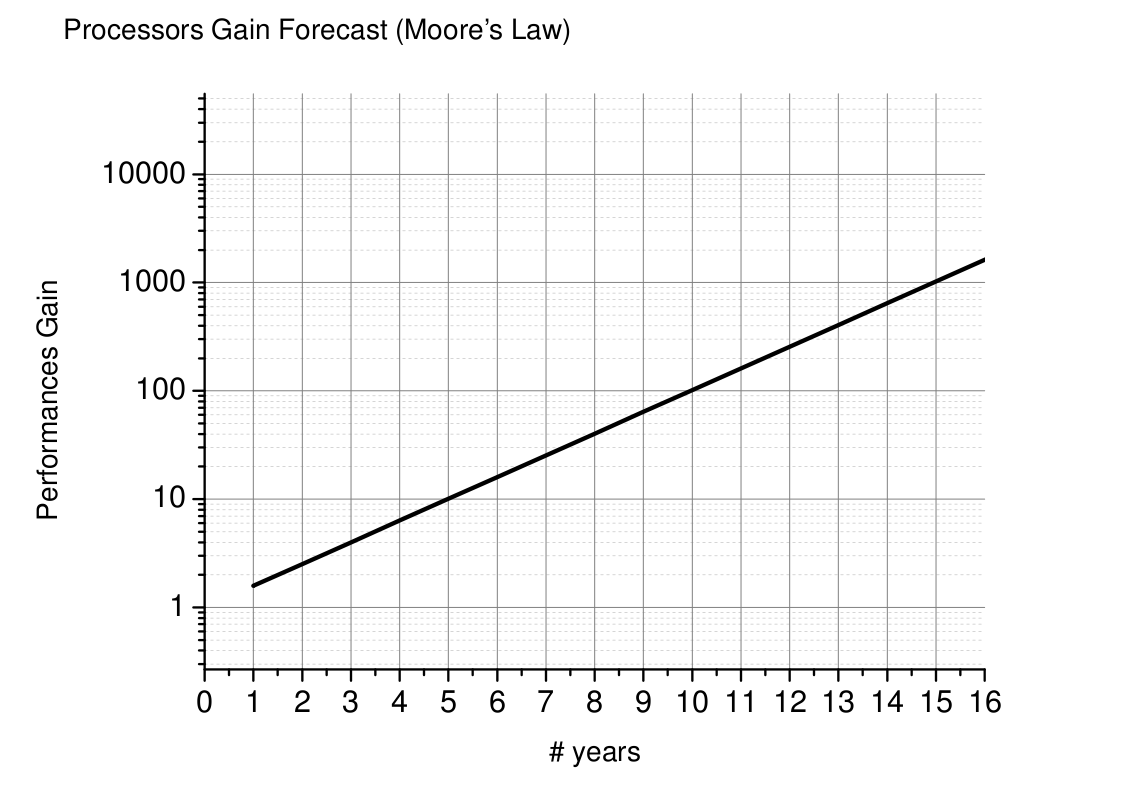
\includegraphics[scale=0.50]{./Sec_ET_ScienceCase/moorelaw.png}
\caption{Moore's law projection of expected computing power gain respect to the epoch of evaluation.}
\label{fig:moorelaw}
\end{figure}


At least up today, this behavior is experimentally proved also by top500 performances graph shown in 
figure~\ref{fig:top500}. As previously noted, the Linpack benchmark is used to rank the system within the list. Thus, 
the values reported in the graph can be considered a good estimation of the real power (i.e.\ sustained performances) 
of the 500 most powerful computer in the world. 

\begin{figure}[h!]
\centering
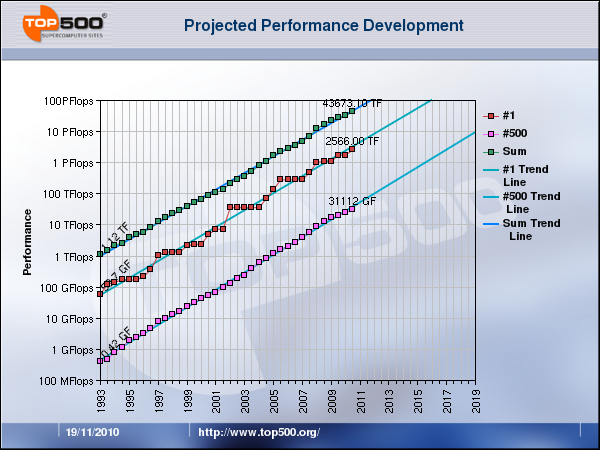
\includegraphics[scale=0.50]{./Sec_ET_ScienceCase/top500graph.png}
\caption{The Top 500 projected performance development (For kind concession of Prof. Dr. Hans
W. Meuer ).}
\label{fig:top500}
\end{figure}

In figure~\ref{fig:top500} are reported three different sequences.
The first one, labeled with {\bf Sum}, represents 
the total amount of computing power of which all the 500 supercomputers in the list are capable. The second sequence, 
the one labeled with {\bf \#1}, is the power of the first ranked system. The last one, the sequence labeled 
with {\bf \#500}, is instead the computing power of the 500-th system in the list. 

A simple execise to show to the reader how the first Moore's law works. If we consider the computing power of the last ranked system
in the list ten year ago, this gives a number of approximately 100 GFlops. Today the 500-th system, namely a Xeon 
Cluster, has a power of more the 10 TFlops. This gives a gain factor of about 100, as the Moore's first law states. So, as it may seem incredible, 
experimental data confirms that in ten years we had and increase of a factor 100.   

%Using the Moore's law it is possible to map also other IT devices, such us Input/Output devices. We report in figure () the expected throughout performaces evolution about hard-disk periferals. 


These information and in particular about GFlops are closely related with computational problem to be faced. In the ET case we can try to select some reference core algorithms and use the our  many-core / Moore's law forecast factor to predict the realistic computing power in 10 years from now. These results can be used to understand the future investigation capabilities and limitation  about some of the main ET data analysis area of interest. 

A fundamental point that distinguish first and second generation gravitational wave detectors  respect to ET science is the nature of the experiment. ET has to possess enough sensitivity and computing power to achieve its main goal, the GW observation and not detection. This means real-timand on-time analysis that will stress the computing infrastructure, requiering the handling of the two main data analysis aspects: detection and parameter recostruction problems.

\FloatBarrier
\subsubsection{Detection Stategies}

{\bf \[Binary~systems\]}  
As shown in the previous sections, binary systems, formed by pairs of neutron stars (NS) or an intermediate massive black hole (IMBH) with another NS or IMBH, are the most important sources for ET \cite{Sathyaprakash2009}. In fact, the detection and the study of IMBH is an astrophysical challenge in itself. 


In the context of full General Relativity, the exact equation describing the gravitational waves emitted by the motion of two compact objects is not really known. The only solution for that problem comes from the Post-Newtonian theory. In this context, a significant progress  had been made in the last few years and now we are able to have waveforms at the $3.5$PN order in phase, $2.5$PN order in  spin-orbit (SO) effect and  $2$PN order for the spin-spin (SS) effects \cite{ARUN2009}.


Two sets of parameters characterize waveforms emitted by  quasi-cicular coalescing binaries % is characterized by two sets of parameters,
:  intrinsic and extrinsic ones. The extrinsic or 
kinematic parameters are all the parameters incorporated in the detection statistic. In our case, they are defined by the inclination $i$, the
polarisation $\psi$ of the source,  the fiducial time of coalescence of the binary $t_c$,  and phase at coalescence $\Phi_c$.  The intrinsic or
dynamic parameters are the reduced mass $\eta$, the chirp mass $M_c$, the algebraic values of the spins $\chi_1$, $\chi_2$ and the sky location of the source $\theta$, $\phi$ (here we consider the algebraic values of the spins since we will limit ourselves to parallel and ant-parallel spins only without including the time evolution of spin directions which will be considered as irrelevant for the purpose of our study).


In addition of these parameters, an other effect which will change the shape of the detected waveform is the Doppler shift effect of the frequency. The detector's motion can no longer be considered as negligible since the observation time could reach few days. This also suggests that a single ET detector could be able to determine the sky location of the source ($\theta$ and $\phi$) even with a moderate precision. 



As the model waveform depends on  number of parameters, the most adequate way to search for the signal is to filter the data through a template bank covering the astrophysically interesting region of the parameter space\cite{owen97, BABAK2006}. It represents a grid of theoretical waveforms (templates) placed, according to a fixed value of the minimal match $MM$, on the parameter space. Each point is associated with a template built from a specific values of the parameters. By matched filtering technique, one finds the maximal value of the likelihood which corresponds to the best mimicking template.


The problem with such technique of search is the large number of templates needed. For an ET-D configuration with a minimum match  of $95\%$ and for a total mass $M$ range $\left[1 M_o~~300 M_o\right]$, the number of templates  roughly ranges from $10^9$ (for templates built using only two parameters : $\eta$, $M_c$ ) %and $10^{13}$  ( for a search with four parameters templates : $\eta$, $M_c$ and an all sky search $\theta$, $\phi$) 
and $10^{18}$ (for spinning binaries  templates wrought by six parametrs : two masses, two angles and two algebraic values of spin), respectively.


In the  Table-\ref{comp.power}, we summarized the computational time needed for a flat search with different number of parameters\footnote{Low cost system in the last column represents computing power features of the smallest top500 system in a couple of years, figure~\ref{fig:top500}. Within ten years, it is  plausible to expect that such a computing capability will be available at an affordable cost}.
\begin{table}[h]
\begin{center}
\begin{tabular}{|c|c||c|c|c|c|c|} 
\hline

\multicolumn{2}{|c||}{Computers} &  GPU C2050 & E@H & WLCG &  Tianhe-1A & Low cost system\\ 
\hline
\multicolumn{2}{|c||}{Processing power (TFlops DP) } & 0.5 & 200 & 2000 &  2567 & 100 \\ 
\hline
 Nbr of para  & Nbr of templ   &  \multicolumn{5}{|c|}{Computational time needed} \\
 \hline
  2   &  $10^9$       & 64 days & 4 hrs  & 24 min   &  18 min  & 7 hrs   \\
 \hline
  4   &  $10^{13}$  & 1760 yrs & 5 yrs   & 182 days   &  128 days    &  9 yrs  \\ 
\hline
   6  &  $10^{18}$  & $179~10^6$ yrs &   $5~10^5$ yrs & $5~10^4$ yrs   & $4~10^4$ yrs  &  $9~10^5$ yrs   \\
\hline
\end{tabular}
\end{center}
\label{comp.power}
\caption{This table gives the computational time needed for a flat search with different number of parameters using : 1 GPU C2050, E@H\ref{EatHbox}, WLCG\ref{Gridbox}, the supercomputer Tianhe-1A and using the performance of the smallest system in the Top500 list in a couple of years, respectively. The results show that using matched filtering search with six parameters template bank or more is not a realistic choice.}
\end{table}


For low SNRs, one could suggest a hierarchical search, looking for a detection at first with a coarse grid and reconstructing the parameters around the detected template with a fine grid template bank in the second pass. However, this could be problematic if we have great SNRs (as in the case of ET). Many templates could have the same maximum value of the likelihood even with disparate values of the parameters (multi-sources, degenerescence). This suggests to use a large parameter space ranges for the second step of search giving a large number of templates, or/and to use a multi-templates search technique (overlap of many sources) where also a huge number of templates is needed. 


The large SNR for ET and the relatively great number of overlapping expected sources  make the most used search techniques, in the case of ground-based detectors, obsolete when  the number of parameters  $N > 4$). Thus, may be the most promising  outcome is to adapt the algorithms used for the future space detector LISA such as MCMC, MHMC or Generics Algorithms (GA) to our purpose \cite{PETITEAU2010}.

Another possible approach can be a two steps  multi-band analysis. In this case the analysis is made first performing a detection phase with templates starting from higher cut-off frequency and assuming a small snr-lost, e.g.\ of about $5\%$. In fact the template length is reduced exponentially starting from highest frequency. Starting for example from 10\,Hz we loose few percent in terms of signal-to-noise but we gain propotionally in terms of computing time.   Thus, the first step can be considered similarly to a trigger zero, used for candidates selection. Then, in the second step, the whole template  is analyzed  for parameters reconstruction and observationi, using a finer template bank grid. Another possible optimization could be achieved using the Stationary Phase Approximation for template production of the first step  and then the PN approximation or others during the second step. This schema can be used also for other kind of generators. 
\\
\\
 
 {\bf \[  Stochastic ~ gravitational~ wave~ background \]}  
The stochastic gravitational wave background could be of cosmological (isotropic---like cosmic microwave background)  or of astrophysical nature (anisotropic following the spatial distribution of the sources).

It could be interpreted as the superposition of a number of plane waves having a frequency $f$ and a certain direction $\Omega$. We assume that the stochastic background is unpolarized, Gaussian, stationary but we allow an anisotropy in its distribution.
The anisotropy of the signal will affect the statistical properties of data with the presence of a signature in the output of the detector \cite{THRANE2009}.
The search methods for each nature of sources should depend on its angular distribution and its spectral properties. 

%Overview of the {\bf isotropic analysis} (the radiometer analysis is almost based on the same framework) \cite{ISOTROPIC1, ISOTROPIC2, RADIOMETER}.


The search for isotropic sources, called {\bf isotropic analysis}, is based on the use of a network of detectors  \cite{ISOTROPIC1, ISOTROPIC2} (the radiometer analysis is almost based on the same framework \cite{RADIOMETER}), where the bulk of the processing time is taken up by reading/writing the data and finding the frequency dependent cross-correlation spectrum and sensitivity. It is done by splitting the output data from several IFOs pairs into short length segments (60 seconds) and performing the analysis (cross-correlation estimation)  for each part separately before summing the partial results at the end.  

%The search for isotropic sources, called {\bf isotropic analysis}, is based on the use of a network of detectors~\cite{ISOTROPIC1, ISOTROPIC2} (the radiometer analysis is almost based on the same framework~\cite{RADIOMETER}). For each detectors pair, first, one searches  the times when both the detectors were taking science data, then split that time up into segments of length $T$ (usually $T \sim 60$ seconds). Let's label the interferometer pair  with an index $I=1, 2, \ldots N$, and for that pair, each segment is labelled by an index $J = 1, 2, \ldots n_{\text{segs}}$. So that, each of the segments analysed can be identified by the unique $(I, J)$ pair. Since the segments will be Hann-windowed, only segments that overlap by 50$\%$ are used.




%The search for isotropic sources, called {\bf isotropic analysis}, is based on the use of a network of detectors  \cite{ISOTROPIC1, ISOTROPIC2} (the radiometer analysis is almost based on the same framework \cite{RADIOMETER}). For each detectors pair, first, one searches  the times when both the detectors were taking science data, then split that time up into segments of length T (usually T ~ 60 seconds). Let's label the interferometer pair  with an index I=1, 2, ... , N, and for that pair, each segment is labelled by an index J = 1, 2, ... $n_{\text{segs}}$. So that, each of the segments analysed can be identified by the unique (I, J) pair. Since the segments will be Hann-windowed, only segments that overlap by 50$\%$ are used.

%The bulk of the processing time is taken up by reading the data and finding the frequency dependent cross-correlation spectrum (the integrand of the cross-correlation estimator statistic, $Y_{IJ}$), and sensitivity integrand (the integrand of the theoretical error bar, $\sigma_{IJ}$) in each unique segment. The steps are:

%Once this has been done one get the cross-correlation spectrum and sensitivity integrand for each unique segment given by the indexes $(I,J)$. Then, the `post-processing' could be started. The last is often repeated several times, without having to re-run the calculation of the spectra.


%\begin{itemize}
%\item read the data for the segment for each IFO,
%\item downsample (to 2048 or 4096 Hz),
%\item high-pass filter to remove low-frequency components,
%\item put the data through a standard PSD estimation function, 
%\item multiply the data with a Hann window,
%\item Fourier Transform the data,
%\item decimate the fourier transform to the same frequency resolution as the PSD (usually 0.25 Hz),
%\item calculate the overlap reduction function at the same resolution,
%\item calculate the optimal filter function,
%\item calculate the cross-correlation spectrum and sensitivity integrand,
%\item write some or all of these quantities to file.
%\end{itemize}


%Once this has been done one get the cross-correlation spectrum and sensitivity integrand for each unique segment given by the indexes (I,J). Then, the 'post-processing' could be started. The last is often repeated several times, without having to re-run the calculation of the spectra.

%For each unique segment $(I, J)$,  the cross-correlation statistic, $Y_{IJ}$  and theoretical error bar, $\sigma_{IJ}$,  are calculated.

%For each pair, one finds the weighted sum of the cross-correlation statistics and theoretical error bars to give combined results $Y_I$ and $\sigma_I$.

%One then finds a weighted sum of the results from the individual pairs, to give an overall statistic $Y$ and error bar $\sigma$. (Note, that normalization is done  such that $Y=\Omega T$, where $\Omega$ is the amplitude of the GW spectrum  \cite{ISOTROPIC1}: % I have to insert a ref to the same equation in the doc

%\begin{equation}
%\Omega = \frac{f}{\rho_c} \frac{\text{d}\rho}{\text{d}f}
%\end{equation} 

%where $\text{d}\rho$ is the energy density of gravitational radiation contained in the frequency range $f$ to $f + \text{d}f$ , $\rho_c$ is the critical energy density of the Universe, and $f$ is frequency.


%{\bf Parallelization:}   One can split the data from each IFO pair into `jobs' which contain several segments (anything up to a few hundred segments).  Then, run the cross-correlation estimation (the items bit) for all the segments in one job on a single node, and these jobs are all run at the same time. So, the analysis which would take 300 hours of CPU time will usually complete within a few hours on the caltech cluster or on atlas. Once all the jobs are completed, they carry out the post-processing (very cheap computationally).

%The final step is to use this statistic to find a Bayesian posterior PDF on the GW amplitude $\Omega$, since this is a one-parameter problem (One marginalizes over any other unknown parameters, such as the calibration factors of the IFOs), one can simply calculate the posterior on a grid % - there's no need to use MCMC or other statistical techniques.

%    - forecast: Stoc. problem size and Computing implications
%    - for 300h x 2months 2pear of interferometers --> ET --> Isotropic/Radiomether --> 30Hour --> 1 Months --> IO Limit
%    - 1h CPU time X 1 Day 
%    Knowing the actual detection algorithm parameterization, it is possible to estimate the computational cost 
%    and foresee the future capabilities give by computing infrastructure improvements. 
%    In particular we can evaluate the cross correlation problem. In this case we know that today the typical 
%    analysis is made in the frequency band 600-10kHz with 0.25 Hz of 
%    frequency resolution. With this information we can deduce the need to use a 20kHz as sample frequency 
%    and in order to achieve a frequency resolution of 0.25 [Hz] we need at least a data vector length of 1/0,25 s = 4 s. 
%    With these information we can estimate the typical data vector length equal to L= 4 x 20000 samples = 80000 samples.




%    - forecast: Stoc. problem size and Computing implications
%    - for 300h x 2months 2pear of interferometers --> ET --> Isotropic/Radiomether --> 30Hour --> 1 Months --> IO Limit
%    - 1h CPU time X 1 Day 
%    Knowing the actual detection algorithm parameterization, it is possible to estimate the computational cost 
%    and foresee the future capabilities give by computing infrastructure improvements. 
%    In particular we can evaluate the cross correlation problem. In this case we know that today the typical 
%    analysis is made in the frequency band 600-10kHz with 0.25 Hz of 
%    frequency resolution. With this information we can deduce the need to use a 20kHz as sample frequency 
%    and in order to achieve a frequency resolution of 0.25 [Hz] we need at least a data vector length of 1/0,25 s = 4 s. 
%    With these information we can estimate the typical data vector length equal to L= 4 x 20000 samples = 80000 samples.

%    If we consider the cross correlation algorithm and 1 Day of data, this computational problem is equal to 
%    perform roughly 43000 analysis cycle x cross correlated channels pair. The total ammount of processed data is 43000 x 8 * 80000 = 26GB per channels pair. 
%    We know that for 1 Day of data we need 1 h of CPU time, thus the estimated IO throughput is about 10MB/s per channels pair.
    
    %%%%
    Knowing the detection algorithm parameterization, it is possible to estimate the computational cost 
and foresee the future capabilities given by computing infrastructure improvements.    %In particular, we can evaluate the cross correlation problem. 

We know that today, the typical cross correlation analysis is made in the frequency band 600-10kHz with 0.25 Hz of frequency resolution. This implies the use of a sampling frequency of 20 kHz and, at least, data vector length of 1/0.25 s = 4 s. Thus, the typical data vector length is equal to L = 4 x 20,000 samples = 80,000 samples. So, for 1 Day of data, one expects to perform roughly 43000 analysis cycle x cross correlated channels pair. The total amount of processed data is, then,  43000 x 8 x 80000 = 28GB per channels pair. 

    We know also that for 1 Day of data we need 1 h of CPU time, thus the estimated IO throughout is about 10MB/s per channels pair.


    Moreover, We can try to estimate the GFlops considering a complexity manly due to FFT algorithm. The FFT complexity is $N\dot log_2(N)$,
    under these hypothesis during a day we have a total value: $Nc~N~log_2(N)$.
    Considering as  FFT reference library the fftw \cite{FFTW},it is possible to show that  this algorithm expresses roghly 6 GFlops for vector data of 80000 sample.

    Now in order to understand if this is a CPU or IO bounded problem we can test the two hypotesis.
    Under the hypotesis of a CPU bounded problem,  we know from the previous evaluation made using real information that now we achieve 1MFlops x pairs channels. This data is 3 order of magnitude smaller than real one.

    Usually the number of cross correlated channels is of the order of some tens, by that it is clear that this kind of analysis seems to be characterized by limitation due to data Input/Output from/to storage. Moreover the CPU power seems to be already enough to process data "in-time".  A faster analysis could be realizing High throughput SAN (Storage Attached Network) 
    
    {\bf Parallelization :}   One can reduce the computational time by splitting the data from each IFO pair into 'jobs' which contain several segments (anything up to a few hundred segments).  Then, run the cross-correlation estimation %(the items bit) 
for all the segments in one job on a single node, and  run all these jobs at the same time. So, the analysis which would take about ten Days of CPU time will usually complete within a few hours using  atlas cluster for example. %Once all the jobs are completed, they carry out the post-processing (very cheap computationally).
   
    
%  From Cornish2001, what it is decomposed in spherical harmonics are the luminosity distribution of the gravitational wave background $L(\theta,\phi, f)$ and the detector response function $F(\theta, \phi, f, t)$. 

%%%%%%
% references Pletsch2009, Pletsch2010

{\bf The sky decomposition method} is used for anisotropic background, the method provides maximum likelihood estimates of the gravitational wave distribution $P(\Omega)$ decompesed with respect to some set of basis functions on the sky \cite{THRANE2009}. This basis could be pixel basis or spherical harmonic basis defined with respect to the Earth's rotational axis.

For point sources the best choice is the pixel basis. However, for a diffuse background dominated by dipolar or quadrupolar distributions, the best choice is the spherical harmonic basis. 

The spherical harmonic analysis method can successfully recover simulated signals injected into simulated noise for several different types of stochastic gravitational wave backgrounds, for examples, isotropic sources, dipole sources, point sources, diffuse sources, etc.


Note that applying the spherical harmonic decomposition   in the case of an isotropic signal, where only the monopole moment contributes to the stochastic gravitational wave background strength function $\Omega_{GW}$ \ref{eq.},  allows to save in computational power and time compared with the isotropic method.

%   One also has to decompose the overlap reduction function with respect to the spherical harmonics.

% In the case of anisotropic stochastic gravitational wave background the likelihood analysis reproduce the matched filtering analysis for isotropic and radiometer, however without introducing the filter function $Q$ into the construction of the statistics. 

%The likelihood estimator for anisotropic background gravitational wave signal is the quantity :

%\begin{equation}
%P_\alpha = (\Gamma_{\alpha \beta})^{-1} X_\beta
%\end{equation}
 

%$X_\beta$ is the components of the dirty map and $(\Gamma_{\alpha\beta})^{-1}$ are the components of the inverse of the beam pattern matrix $\Gamma_{\alpha\beta}$. It plies a role similar to that of the Fisher matrix. For spherical harmonic decomposition, the index $\alpha$ corresponds to the couple $l,m$.

%%%%%% begin
%%%By fixing the shape of the gravitational wave background (initialize the value of the reference frequency where the detector is most sensitive and the index of the power-law behavior of the gravitational wave spectrum) 
%%%%%% end

%\begin{equation}
%X_\beta = \sum_t \sum_f \gamma_\beta^*(f,t) \frac{\tilde{H}(f)}{P_1(f,t) P_2(f,t)} C(f,t) 
%\end{equation}

%\begin{equation}
%\Gamma_{\alpha \beta} =  \sum_t \sum_f \gamma_\alpha^*(f,t) \frac{\tilde{H}(f)}{P_1(f,t) P_2(f,t)} \gamma_\beta(f,t)
%\end{equation}


%The different functions appearing in the above formulas are defined and computed as following \cite{THRANE2009}:

%\begin{itemize}
%\item The input $\tilde{H}(f) = (f/f_R)^\beta $ is the assumed spectral shape of the gravitational wave background. It is fixed at the start of the analysis by initializing the value of the reference frequency $f_R$ (the most sensitive frequency) of the detector and  the spectral index $\beta$ for the power-law behavior of the gravitational wave spectrum (note that $\beta=0$ corresponds to a constant gravitational strain power.
%\item  $C(f,t)$ is the cross-spectra of the data calculated as the SFT of the time-series output data of the two detectors :
%\begin{itemize}
%\item down-sample output data to few  kHz.
%\item high-pass above few Hz to reduce contamination from seismic noise.
%\item windowed.
%\item discrete Fourier transformed to frequency domain. 
%\end{itemize}
%\end{itemize}
%Note that the frequency resolution ($0.01$ Hz) for $C(f,t)$ is much smaller than that one for $\tilde{H}(f,t)$ or for the spectral density function $P_i(f,t)$ ($i=1,~2)$ and $\gamma_\alpha(f,t)$ which is fixed to $0.25$ Hz. This is used to avoid unnecessary frequency resolution for these last functions, by averaging several frequency bins of $C(f,t)$ before  to match $\Delta f$.

%\begin{itemize}
%\item $P_i(f,t)$ ($i=1,2$) are the power spectra associated with the individual detectors computed according to Welch's modified periodogram using segments of 4-sec long ($0.25$ Hz) and $50\%$ overlapping.
%\item $\gamma_\alpha(f,t)$ are the components of the overlap factor $\gamma(\Omega, f,t)$. they encode informations about the relative separation and orientation of the detectors as expressed by their beam pattern functions. They are analytically computed in the case of spherical harmonics decomposition.  
%\item Choose a cutoff for the SVD regularization (fixe minimum eigenvalues  for which the Fisher matrix is reversible). %%% check
%\item Choose $l_\text{max}$. It consists of tradeoff between increasing the number of parameters to fit the data and  minimizing the uncertainties. 
%\end{itemize}



However, in general,  this method is more computationally intensive than isotropic and radiometer methods.  The computation time will be proportional to some function of the maximum value $l_\text{max}$ of the modes, but roughly estimates show that the spherical harmonic search takes 10 times as much CPU time as the isotropic/radiometer searches.
    
    
    
    
{\bf \[Continuos ~Waves~ Analysis\]} We clasify as continuous waves (CW) a gravitational wave signal with duration longer than the typical observation time of a detector. The signal of these sources could be affected by a various processes. (i)~By spin-down: the rotation frequency and then the emitted signal frequency slowly decreases due to the energy loss of the source (EM, GW, \dots). (ii)~The signal is frequency modulated by the Doppler effect associated to the relative source-detector motion. (iii)~ Signal is amplitude modulated due to the non-uniform antenna sensitivity pattern of the detector.  (iv)~There are also two further complications that can affect the GW signal from real sources : glitches which are brief spin-up due to star-quakes or interactions between crust and superfluid and timing noise which is random fluctuations of the rotation frequency or phase. 

The analysis methods for CW can be divided among coherent, i.e.\  that take into account the signal phase when known (matched filtering, cross-correlation, MCMC) and incoherent, where the signal phase is discarded (periodogram,  Hough transform).
Typically, incoherent methods are more robust and less computationally demanding even less sensitive. 

The choice of a method   depends closely on the prior information we have on the signal we are searching and on the available computing power. We can distinguish between two kinds of cases : 
\begin{itemize}
\item Targeted search : cases where knowledges about the source parameters (position, frequency, spin-down) are available from electromagnetic observations of the source.
\item Blind search : cases where all the source parameters are given within large intervals based on the available theoretical understanding of the astrophysical scenarios. 
\end{itemize}

The targeted search could be schematized as following: (1)~Extract the band of interest around the emission frequency: due to the Doppler effect, the amplitude modulation and the spin-down, the received GW is no longer monochromatic and covers a small  frequency band (fraction of Hz) around the twice electromagnetic frequency.  (2)~Correct Doppler and spin-down effect : if the spin-down parameters of a source are known with high accuracy we can remove both the Doppler and spin-down by multiplying data by an appropriate function. %the proper function $exp(-I~\Delta \Phi_{\text{Doppler, spin-down}})$. 
(3)~Matched filtering: apply matched filter of the new slowly varying signal (demodulated signal) over the unknown nuisance parameters (amplitude of signal as received on Earth, polarization and inclination angles, initial phase\dots) and over the uncertainty range of the known parameters (position angles, frequency, spin-down).  An alternative to explicitly apply a matched filter for the nuisance parameters is the use of the so-called F-statistics~\cite{ItohFStatistic}. (4)~Select maximum of the values of the unknown parameters at filter output. (5)~Compare it with noise distribution and claim detection or set an upper limit.  %  make it more clear (5)

The computational cost for targeted searches relies on the accurate knowledge of the source parameters: position, frequency, spin-down.
Considering that the frequency is very accurately known within a small bandwidth, one can  easily down-sample the data stream around the expected source frequency and  the data analysis cost for such sources is therefore minimal (few templates). However, even for sources observed in the electromagnetic domain,  these parameters are known with finite accuracy and this can lead to a loss of sensitivity, especially for very long observation times. This will also  increase the computational cost. 

In the case of NSs for which no substantial information about the spin-domw parameters are known, the computational cost is more important. From one side,  it is no longer possible to set an upper-limit on the signal strain. And  from the other side,  It is obvious that, because of the lack of information about the higher spin-down parameters,   one would also have to scan their parameter space. The number of templates is then in the range  $10^2~ - ~  10^{10}$, for a year's worth of integration  \cite{DhurandharCW}. Therefore, even if we perform the search in a narrow frequency band around twice the radio pulsar frequency, the computational task is really tricky.
 %For those NS's about which no information about the spin-down is available, we cannot set upper-limits on the signal strain and hence the computational cost becomes considerable. The number of templates is in the range  $10^2 -  10^{10}$, for a year's worth of integration  \cite{DhurandharCW}. Therefore, even assuming a search in a narrow frequency range, around twice the radio frequency, the computational task is tricky. The situation is made worse by the lack of information about the frequency time derivatives, so that one would also have to scan the space of spin-down parameters, increasing the cost further. 
Thus, It is clear that more accurate data from radio observations are necessary in order to narrow down the uncertainty in the source parameters for making such searches feasible.

These results suggest also that applying matched filtering method for a blind search is computationally not possible, since the minimal range for the source parameters is important (whole sky for angular position,  whole bandwidth for the signal's frequency\footnote{The computational power is proportional to the maximum frequency of the detector to the fourth power~\cite{DhurandharCW}} \dots).  Even for the more optimistic cases, the computational power required for such search is far from our actual computational capabilities ( $10^{17}$ GFlops for circular orbit binaries). A different approach with even a small loss of sensitivity but which ensures to reduce significantly the computational power is then needed.


%{\bf Stack-slide}  % =======> CW after coherent and uncoherent search 
% However Badri is working on this section 
One of the solution is the so-called hierarchical search ({\bf stack-slide search} \cite{BRADYbis}) where coherent and incoherent steps are alternated. In the incoherent step a rough exploration of the parameter space using short data segments is done with a low threshold which allows for many false alarms (some candidates are selected). In the coherent step each candidate is followed with a more refined search using long data segments but searching the parameter space only in the neighborhood of the detected candidates of the first step.



Both search steps considered above share the following scheme \cite{BRADY1}: 
\begin{itemize}
\item The output data are divided into short segments, called stacks.
\item Each segment is phase corrected using an appropriate mesh of correction points to confine an alleged signal in one frequency bin.
\item Fourier Transform the phase corrected stacks
\item Using finer mesh, the individual power spectra are corrected for residual frequency drift by removing phase modulations over the entire data stream.
\item Sum the corrected power spectra.
\item Search for candidates exceeding some fixed thresholds.
\end{itemize}

%Both search steps considered above share the following scheme \cite{BRADY1}: first, the data stream is divided into shorter lengths, called stacks. Each stack
%s phase corrected and FFT'ed, using a mesh of correction points sufficient to confine a putative signal to $\tilde{1}$ frequency bin in each stack. The individual power spectra are then corrected for residual frequency drift using a finer parameter mesh suitable to remove phase modulations over the entire data stretch. The corrected power spectra are summed, and searched for spikes which exceed some specified significance threshold.

From the computational point of view, the interesting feature of stack-slide method is the fact that it considers the available computational power as an initial parameter which fixes the values of the other parameters of the scheme. In fact,  before the search begins, one has to specify the size of the parameter space to be searched (choose maximum frequency,  region of the sky \dots), the available computational power to do the data analysis, and an acceptable false alarm probability. From these, one can fix optimal values for the maximum mismatch for a patch, the number and the length  of stacks. Optimization consists of maximising the sensitivity function over these parameters given the definition of the total computational power as constraint.

The advantages of a hierarchical search are, from one hand the fact that the low threshold on the first step allows detection of low-amplitude signals which would otherwise be rejected, and from the other hand the second step can search longer data slices on a limited computing budget, because of the reduced parameter space being searched, thus excluding false positives from the first pass. For given computational resources, this technique achieves the best sensitivity if the thresholds and mesh points are optimally chosen between the first and second step of search.

% An other possible alternative approach is e.g.\ proposed by .......... make a good connection 

%Wide-area searches for continuous gravitational signals emitted by rotating neutron stars is an hard task and it 
%cannot be addressed using optimal data analysis methods, due to the huge computational power needed.

Another possible alternative approach is e.g.\ proposed by \cite{}%(PHYSICAL REVIEW D, VOLUME 70, 082001)(Quantum Grav. 22 (2005) S1255.S1264), 
where thay developed a hierarchical method
allowing a cut of  data analysis computational requirement. This method is sub-optimal and the processing gain is paid by a small
reduction in sensitivity. The method consists mainly on alternating coherent steps, based on FFT, and incoherent steps 
based on the {\bf Hough transform}. The Hough transform  is a feature extraction technique used typicaly  in image analysis, 
computer vision, and digital image processing. The purpose of the technique is to find imperfect instances of objects 
within a certain class of shapes by a voting procedure. This voting procedure is carried out in a parameter space, 
from which object candidates are obtained as local maxima in a so-called accumulator space that is explicitly 
constructed by the algorithm for computing the Hough transform.
In paper \cite{} %(Quantum Grav. 22 (2005) S1255.S1264)
 the computational requirements for a search over these many 
templates is also estimated. Analyzing the data in roughly real time requiresa computational power $10^8$GFlops, 
moreover is reported the performances of the  fastest supercomputers ca. 2010, $5\dot10^4$GFlops.

Considering a foreseen factor of 200 we can expect in 2023 that the fastest super computer is capable of $10^7$GFlops. This number is still an order of magnitude lower and we can conlude that with type of analysis the online will be still not achievable.

%- Power Flux (Sofiane)
%- forecast:Cont. wave problem size and Computing implications
%
%(Unmodelled sources) todo: set references
%    ("Gravitational waves from r-modes" Paulo M. S� � Brigitte Tom� - Astrophys Space Sci (2007) 308: 557.561
%    ("Gravitational waves from the r-modes of rapidly rotating neutron stars" Owen B.J.  - Gravitational Waves, AIP Conference Proceedings, Vol. 523. New York: AIP Press, 2000., p.55 

 {\bf \[  Unmodelled~sources \]}  
{\bf [R-Modes]}~After the supernova event, the newborn neutron star may spin down during up to one year due to R-modes instability. R-modes are non-radial pulsation modes of rotating stars that have the Coriolis force as restoring force with a characteristic frequency comparable to star rotation speed.
    These modes are driven unstable by gravitational radiation, inducing a differential rotation at second order in mode's amplitude, which leads the non linear evolution of the r-mode instability. This process generates gravitational waves that are very difficult to be observed.


    R-modes gravitational waves are interesting for ET Science, because could provide very foundamentals information about Formation Processes, such as initial condition, Neutron Star model and Equation of State and others like Neutrino emission models confirmations.  In some sense R-mode gravitational wave observation can produce important and unique correlation with the nuclear physics of the neutron star and formation processes.  

Using information reported in (Sa and Tome  model - P. M. Sa and B. Tome - Astrophys Space Sci (2007) 308: 557.561) we can acquire some characterizing data about this type of signals. 
    The frequency domain of these waves is related to the angular velocity $W$ by: $f=2W/(3p)$.  The frequency bound is given
   \begin{itemize}
    \item fmax $\sim$  1200 Hz, it depends on the initial value of the angular velocity $W0$
    \item fmin $\sim$ (77-80) Hz, it depends on the final value of the angular velocity $W(tf)$ and $K$
    \item The GW duration is roughly $tf =(3.6 - 7.1)10^6 s$
   \end{itemize}
 
    In ((Sa and Tome model)) is also reported the Gravitational waves strain h(f) generated by R-mode:
    (formula)     %%%  missing formula      <================((((((

    We estimate the optimal signal-to-noise ratio for Einstein Telescope case, and it is given by the formula:
    \[\frac{S}{N} = \frac{200}{\sqrt{2+K}}\frac{20Mpc}{D}\]
    
    Given these results, we can make hypotesis about the ET horizon respect to rmodes gravitational waves. On douing that we consider the best and pessimistic cases realted to a very high $K$. Thus, if a NS borns with substantial differential rotation of $K= (10^5- 10^6)$ the ovserved optimal SNR is about $[4-12] @1Mpc$. While if $K=0$ we achieve $120Mpc$ close to GA.

    
{\bf Burst Analysis}~Currently, there are two successful methods for searching burst events: Omega and coherent wave burst (cWB). 
With cWB, the basic idea is to combine coherently  time-frequency (t-f) maps from several detectors \cite{KLIMENKO2011}. The sky position is encoded in the time  delays between  interferometers. If there was no time delay, then excess of power in some pixels in t-f map should be  similar (modulo the antenna pattern). So one can determine the sky location of the  signal from the antenna pattern and by doing multiple time shifts of the data corresponding  to different sky positions. %(The basic paper is Klimenko, Mohanty),

%Doing analysis with networks of 2, 3,... detectors, the computational cost will not be very different since
The number of detectors does not affect  the computational cost since we do not analyze data from each detector separately but generate triggers on combined data stream. %So adding another detector should not be an issue by itself.  
However, if we do joint analysis with LIGO and Virgo detectors, there is no point to combine the data if the sensitivity is very uneven (the weakest detector will bring noise to the analysis). In this case,  it only makes sense to use the bandwidth where all detectors are reasonably sensitive. This would probably reduce the bandwidth of ET. At least,  we can subdivide bandwidth into regions with comparable sensitivities and analyze each separately. If ET sees something but LIGO and Virgo do not, it would effectively be 1-detector analysis with no way to find the sky coordinates.

Recent use of that method in case of signal given by noise and glitches only (no gravitational waves),  the computational cost is trivial. To process two years of S5 for 3 detectors with triple coincidence duty cycle of  $40\%$, it would just take one week  on Atlas cluster ( 80 TFlops\footnote{Atlas is composed by 1680 2.4GHz 64bit quad core CPUs which sums up to 64TFlops and 132 Tesla graphic cards which gives us a theoretical peak performance of  132TFlops. The real power processing of Atlas is less than the half of its peak value.}) if it is not too loaded or broken. Also, during S6,  burst search was run online for H1,L1,V1 producing coherent triggers about 5 minutes behind the real time doing computation on 1 dedicated computer. However, in the ET era there might be such a rate of events that it becomes much more computationally intensive. Also if each event is long duration or wide bandwidth, it might consists of millions pixels. Processing such huge clusters might be quite computationally intensive, however still feasible with the future computational configurations.

Finally, one can emphasis that the computational cost for cWB search  depends on which detectors, what frequency band one want to explore and based on this one could estimate how many sky locations he can/should consider.
 But practically, the most important factor is the large false alarm rate that could not be predicted before the detector is switched on. If some detector is glitchy, that might increase computational cost a lot since one would have to consider a lot of huge glitches before finding that
they are inconsistent in some way.

Note that for these kinds of search only sky location and the gravitational strength of the gravitational burst could be recovered, however, the likelihood method used in the search offers a convenient framework for introduction of constraints arising from the source models \cite{KLIMENKO2011}. In fact one of the   constraints is related to the different polarization states of the GW signals. For example, linear or random polarization is predicted for  some of core collapse models \cite{LINEARPOLAR}. Merging compact binaries    produce, in principal,  elliptically polarized gravitational wave signals \cite{RANDOMPOLAR}. Also relativistic jets are emitted along the rotational axis of binary systems during the merger of neutron star, and where circular polarization of the gravitational waves is expected \cite{MERGINGBIN}.  The cWB algorithm allows searches with several types of the polarization constraints : circular, linear, elliptical and random, or un-modeled search\cite{KLIMENKO2011}. Moreover, joining these results with neutrino observations will probably give a powerful tool to probe the physical scenarios behind such kind of sources. 



For {\bf modeled bursts} like GRBs from both core collapse,  supernovae and some of mergers, the search is based on a matched filtering variant so-called time sliced matched filtering \cite{MAURICE2011}.  The application of matched filtering depends crucially on phase coherence in the true signal, in correlating it to a model template.  To circumvent phase incoherence on long time scales created by turbulence in the inner disk or torus of magneto-hydrodynamical systems powered by Kerr black hole,   
the template is sliced  into several segments on intermediate time scales, for which phase-coherence may be sustained.
 Matched filtering is then applied using each slice, by correlating each template slices with the detector output with arbitrary offset  in time.
The relevant parameters in this algorithm are three: a choice of coherence time  which can be  course grained, fine grained time of onset(s) of the (slices of the) burst and the mass of the black hole. The mass is equivalent, for all practical purposes, to the duration of the burst. Changing the black hole mass changes the duration and also the  strength of the signal, but the latter is automatically absorbed by the algorithm and requires no adjustments.  
For this kind of search, a computational cost can be extrapolated. For a single black hole mass parameter, it is about 6 hours of CPU time (core 2 duo) per 1 hour of detector data (sampled at 20 kHz). For a range  of black hole parameters with, e.g.\ , 0.1$\%$ partition, a full parameter search amounts to a few thousand  hours per 1 hour of detector data. In this case we can expect for about 2013  a gain factor of 200 considering the same architecture. Implementing Many-core tecnology factor we can consider a conservative 6 extra-factor (1200). The full parameter search will be roughly 10 times far from the "in-time" constrain using a "CPU" model, while trying a many-core implementation few hours of data will be analyzed in one hour. Thus for about  2014 the "in-time" analysis of full parameter search could be reasonable.          


{\bf [Reconstruction]}
The genetic algorithm (GA) is a search technique that mimics the process of natural evolution based on the positive mutation principle.
Initially, a group of organisms (templates) is chosen, each organism is characterized by a different set of genes (parameters). Then, the quality (log of the likelihood) of each organism is evaluated. Based on the value of their quality (templates with higher likelihood), a set of pairs (parents) are selected and their genotypes are combined to produce  children (new templates). In the last step, one could, with a controlled probability, allow random mutations in the children's genes (by randomly changing the parameters of the new template to explore a large area of the parameter space). The new children will form the new parent and the procedure is repeated until one reaches steady state (maximum in the log likelihood).
From the computational point of view and for the case of coalescing binaries, one could be able to recover the values of the coalescing time and the chirp mass in 1 hour of time with 1 CPU. For the other parameters except the direction of the spins 10 hours of time is needed with 100 CPU. An all parameters recovery will need  few days of time with 100 CPU.
The cost is purely dominated by the computation (time domain $+$ FFT) of the templates (1 to 2 sec with 1 CPU for a waveform lasting 2 years).
\FloatBarrier
\subsubsection{Conclusions}

%-- Observation Feedback on Theory
%-- open to new algotithms possibility
%-- Finally we would like to stress again that: to properly exploit the full power of the new incoming computing
%   architecture, a great effort on the software side is strictly needed, regardless of the architecture we will 
%   use. 

The most plausible computing scenario of the near future is a combination of CPU and GPU technologies, an evolution of most recent AMD's APU or Intel's Knight ferry technologies.  We already showed that it is possible to exploit GPU power in Coalescing Binaries Detection. That means that manycore programming will not be a choice, because will be the status of art at the ET era. This consideration has permitted to add and extra gain factor to the Moore's law expected performances. In general we can consider a base gain factor of 200 by 2023 due to Moore's law and a manycore extra factor that can oscillate, depending on the analysis  that can be posed conservatively  to 10.
This means a potential gain of more than 3 orders of magnitudes.

Given the computing power forecast, we believe that, if we discard a flat search approach with more than 4 parameters and the  search for CW with great number of spin-down parameters (where more sophisticated improvements should be done), the combination of  existing search methods and the future improvement of computing resources will allow  ET to fully  take advantage of its technological design and to play its real role as telescope giving the scientist community the expected information to explore the universe with new eyes.

We should also mention emerging technologies for distributed computing, such as: Grid and Cloud computing facilities. Here the Seti@H, E@H, LHC@home experiments are a great example. These will follow the evolutionary trend and will provide an important CPU power containers for off-line analysis.

We would like to conclude remarking that, technological breakthroughs are taking place. The computing infrastructure trend is toward manycore solutions, as show by top500 and manufacturers road-maps. The possibility to address future computing power for ET science needs will be proportional on how we will be able to use these new architectures. The doubling of performances each 18 months is no more for free. A change on programming paradigm and coding will be mandatory.




\FloatBarrier
% Nomenclature - How it works ?
%where nom_class can be one of a (for abbreviation) g (for glossary) or s (for symbol), nom_label is key word or symbol that you are trying to expand or explain and nom_text is simply the explanation. Optionally nom_class can be followed by a sort word that latex should use to sort (which can be helpful in the case of symbols).
%
% \nomenclature[gC]{Compact star}{ Throughout this document a compact star stands for a neutron star or a black hole}
% \nomenclature[]{}{ }
%
%Computational changllenges file
%
% ======== Nomenclature ==========================================================
%
%Digital Enterprise Group (DEG)





